\documentclass[aspectratio=169]{beamer}
%\usepackage[utf8]{inputenc}
\usepackage[square,numbers]{natbib}

\title{Natural Language Processing: Final Project}
\author{Juan David García\\
César Garrido\\
Nicolás Rocha}
\date{May 2021}

\begin{document}

\begin{frame}
    \maketitle
\end{frame}

\begin{frame}{Agenda}
    \tableofcontents
\end{frame}

% ------------------------------------------------------------
%                             DATA
% ------------------------------------------------------------

\section{Data Recollection}
% Fuentes y cómo se recolectó cada una (ejemplos)
% Formato de almacenamiento
% Estadísticas

\begin{frame}{Reddit}

\begin{figure}[H]
    \minipage{0.5\textwidth}
    
    \begin{figure}
    \centering
    \includegraphics[trim=0cm 10cm 0cm 10cm, clip=true, width=0.5\textwidth]{images/reddit_logo.jpg}
\end{figure}

\begin{itemize}
    \item Downloaded data using PRAW (Python Reddit API Wrapper).
    
    \item Search done in Covid related subreddits:
    \begin{itemize}
        \item \textbf{EN:} r/Coronavirus, r/Covid19
        
        \item \textbf{ES:} r/Coronaspain, r/covidmx
        
        \item \textbf{FR:} r/CoronavirusFrance.
    \end{itemize}
    
    \item Downloaded information not only from \textbf{posts} (new, hot, top), but from \textbf{comments} too.

\end{itemize}

    
    \endminipage\hfill
    \minipage{0.5\textwidth}
    
    \begin{figure}
        \centering
        \includegraphics[width=0.9\textwidth]{images/reddit_example.png}
    \end{figure}
    
    \endminipage\hfill
\end{figure}

\end{frame}


\begin{frame}{Twitter}
    
    \begin{figure}[H]
    \minipage{0.5\textwidth}
    
    \begin{figure}
    \centering
    \includegraphics[width=0.5\textwidth]{images/twitter-logo.png}
\end{figure}

\begin{itemize}
    \item Downloaded data using Twitter API v2.

    \item API allows to set rules explaining what the user wants to find: value, retweet, media, tags, username, links, language, dates, etc.
    
    \item The request contains the rules as well as the desired information per tweet.
\end{itemize}

    
\endminipage\hfill
\minipage{0.5\textwidth}
\begin{itemize}
    \item The request can be done retrieving recent tweets or live tweets. No full-archive access was granted.
    \item All team members requested developer access in order to download tweets simultaneously.
    \item Mainly the live connection was used to retrieve tweets in the three languages.
    \end{itemize}
\endminipage\hfill
\end{figure}


\end{frame}


\begin{frame}{Data recollection: News}
    \begin{columns}
        \column{0.6\textwidth}
            \begin{itemize}
                \item Defined search parameters: languages, countries, keywords and dates.
                \item Called the \texttt{pygooglenews} API with search parameters to acquire news metadata: title, URL and source.
                \item Retrieved news source HTML using the \texttt{urllib} module from Python. 
                \item Data was firstly stored in JSON format and then zipped to reduce disk storage consumption.
                \item In order to speed-up recollection a pool of threads was implemented.
            \end{itemize}
    
        \column{0.4\textwidth}
            \centering
            \includegraphics[width=0.6\textwidth]{images/google_news_logo.png}
            \begin{table}[h]
                \centering
                \begin{tabular}{c|c}
                    \textbf{Parameter} & \textbf{Count} \\
                    Countries (EN) & 19 \\
                    Countries (ES) & 21 \\
                    Countries (FR) & 31
                \end{tabular}
                \label{tab:label_for_table}
            \end{table}
    \end{columns}
\end{frame}

\begin{frame}[fragile]{Data recollection: Data Format}

\begin{itemize}
    \item All docs are saved in the same \texttt{.json} format.
    
    \item Some sources include more keys than others, but all have at least the following information:
\end{itemize}

    \begin{lstlisting}[language=json,firstnumber=1]
{
    "source": "twitter",
    "lang": "en",
    "date": "2021-04-04 19:52:11",
    "author": "mets_rant",
    "text": "@timbhealey Watch the Phillies get covid now",
    "url": "https://twitter.com/anyuser/status
    /1378797568491192332"
}

\end{lstlisting}
\end{frame}

\begin{frame}{Data recollection: Statistics}
    \begin{table}[]
    \centering
    \caption{Total documentes retrieved per language}
    \label{tab:my-table}
    \begin{tabular}{lcccc}
    \hline
    \textbf{Language} & \textbf{Reddit} & \textbf{Twitter} & \textbf{News} & \textbf{Total}\\ \hline
    English           & 297.736   & 651.761          & 447.754          & 1'397.251 \\ \hline
    Spanish           & 9.150     & 245.664          & 257.754          & 512.568\\ \hline
    French            & 4.682     & 121.400          & 699.669          & 825.751    \\ \hline
    \textbf{Total}  & 311.568   & 1'018.825         & 1'405.177 \\ \hline
    \end{tabular}
    \end{table}
    
\end{frame}

\begin{frame}{Data recollection: Statistics}
    \begin{figure}
        \centering
        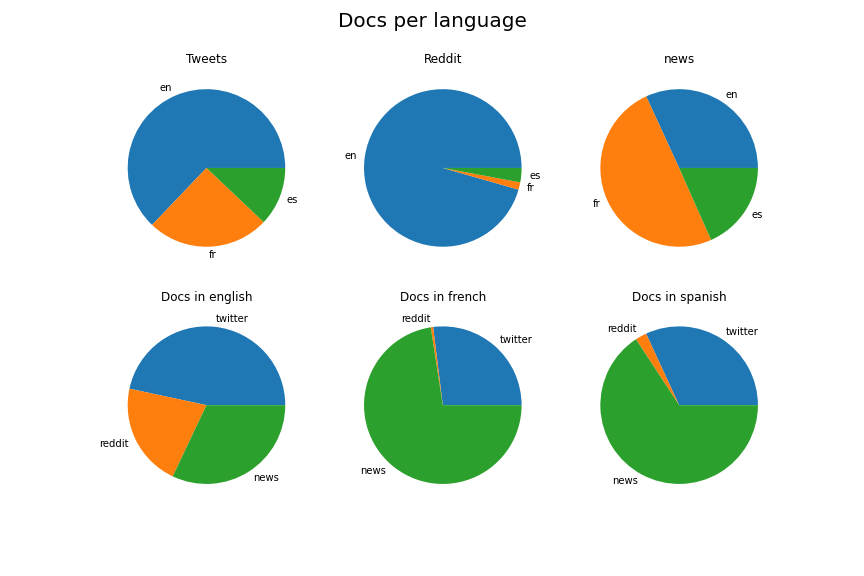
\includegraphics[scale=0.4]{images/total_data.png}
        \caption{Caption}
        \label{fig:my_label}
    \end{figure}
\end{frame}

% ------------------------------------------------------------
%                    P1: Trending Topics
% ------------------------------------------------------------
\section{Automatic Detection of Trending Topics}

\begin{frame}{Topic Detection: State of the Art}

\begin{itemize}
    \item In \cite{ReviewApproachesTopcicDetection} a review of different approaches for topic detection in Twitter is presented (2020):
    \begin{itemize}
        \item \textbf{Traditional medias:} Document-pivot vs. feature-pivot.
        
        \item \textbf{Embeddings:} without (BOW, Tf-idf, NER enhanced, Metadata, LDA, etc.) vs. with (Word2Vec, pretrained word embeddings, contextual word embeddings).
        
        \item \textbf{Detection Techniques:} Classification based (supervised) and Clusstering based (unsupervised).
    \end{itemize}
    
\item \cite{TrendTopicsDetectionFromTwitter} and \cite{FuzzyIncrementalTopicDetection} present different approaches to topic clustering and trend description (extracting keywords from documents).
    
\item  \cite{DeepRepresentationClusteringTweets} and \cite{UnsupervisedDeepEmbeddingClustering} showed that encoder representations (from trained autoencoders) can improve significantly the clustering task.
\end{itemize}

\end{frame}

\begin{frame}{Topic Detection: Our proposal}

\begin{figure}
    \centering
   \includegraphics[width=\textwidth]{images/TopicDetection.png}
\end{figure}

\end{frame}

%\begin{frame}{Topic Detection: Preliminary Results}

%\begin{itemize}
%    \item Data: 5 Categories from Reuters dataset
    
%    \item Model: DestilBert
    
%    \item Embeddings: Only Last Layer
%\end{itemize}

%\end{frame}


% ------------------------------------------------------------
%                  P2 & P3: Doc Classification
% ------------------------------------------------------------
\section{Automatic Identification: Document Classification}
\begin{frame}{The Document Identification Task}
    \begin{columns}
        \column{0.6\textwidth}
        \begin{itemize}
            \item We will address the identification of documents with specific topics as a classification task. Both the binary classification and a multi-class classification tasks will be explored.
            \item Two groups of documents will be assumed as the positive class: the vaccines, vaccination and mental health group, and the school-reopening and house-hold violence group.
        \end{itemize}
        
        \column{0.4\textwidth}
        \includegraphics[width=\textwidth]{images/doc_class_folder.png}
    \end{columns}
\end{frame}

\begin{frame}{Document Classification: State of the Art}
    According to \cite{DC_SPRINGER} document classification consist of assigning a label to a document from a predefined set of labels. Several datasets and approaches have been presented by research groups in order to asses the document classification task. We will consider the following state-of-the-art work in order to solve the automatic identification task:
    \begin{itemize}
        \item \cite{DC_REUTERS} achieved a 97.44\% accuracy on the Reuters-21587 dataset using Message Passing Attention Networks for Document undertanding (MPAD). MAPD is a specific type of Graph Neural Network used for natural language processing.
        \item \cite{DC_BERT_ELMO} uses both BERT and ELMo to classify documents from ten biomedical and clinical datasets. The model with the best performance was a BERT model that was pre-trained with biomedical datasets instead of the the general pre-trained model.
    \end{itemize}
\end{frame}

\begin{frame}{Document Classification: State of the Art (cont.)}
    \begin{itemize}
        \item \cite{DC_DOCBERT} presents docBERT. The docBERT approach consists of distilling a BERT model into a LSTM model. By distilling the model the parameters count is reduced by 30 times thus decreasing the model complexity. The resulting LSTM model is able to classify documents trailing the BERT metrics by 3\% at most.
        \item \cite{DC_REG_EMBEDDING} introduces a comparison between regularized and non-regularized word embeddings. The approaches were tested on a kNN classifier used over six different datasets. An average test error reduction of 39\% was identified by using the regularized word-embeddings.
    \end{itemize}
\end{frame}

\begin{frame}{Document Classification: Our Proposal for Tagging}
    \begin{itemize}
        \item Test runs will be performed on known document-classification datasets such as Reuters-21587.
        \item We will rely mostly on the news dataset to solve the classification problem.
        \item News dataset include a \texttt{keyword} field which will be used as a label.
        \item An attempt on inferring classes from social media documents will be made.
    \end{itemize}
\end{frame}

\begin{frame}{Document Classification: Our Proposal for Classification}
    \centering
    \includegraphics[width=0.8\textwidth]{images/doc_class_naive.png}
\end{frame}

\begin{frame}{Document Classification: Our Proposal Specifics}
    \begin{columns}
        \column{0.5\textwidth}
            \textbf{Document Representation}
            \begin{itemize}
                \item The document representation will be generated from either a pre-trained BERT model or a regularized embedding.
                \item A baseline representation will be used as a reference for determining the improvement over both approaches.
            \end{itemize}
        
        \column{0.5\textwidth}
            \textbf{Classifier}
            \begin{itemize}
                \item Literature review suggested that the classifier architecture/method has not major influence over results. Other tasks found the same suggestion.
                \item A pool of classifiers will be used: Fully Connected Networks and Recurrent Neural Networks
            \end{itemize}
    \end{columns}
\end{frame}


% ------------------------------------------------------------
%                        P4: Q&A System
% ------------------------------------------------------------
\section{Q\&A System}

\begin{frame}{Q\&A System: State of the art}
    \begin{itemize}
        \item \textbf{Q\&A System?} In a question-answering task, the model typically answers a question based on a context (additional text) by marking \textit{the beginning} and \textit{the end} of the answer in that context. 
    
        \item State of the art Q\&A Systems use contextual pre-trained NLP models such as BERT \cite{BertQA}. Pretraining is done for this specific task with datasets such as SQuAD \cite{squad}. HuggingFaces provides a pipeline for Q\&A with DistilBERT \cite{9DistilBERT}.
        
        \item \textbf{How to select the context?} Ranked Information retrieval: RRI, RRDV or even Deep Arquitectures \cite{DeepRanked}.
    \end{itemize}
\end{frame}

\begin{frame}{Q\&A System: Our proposal}

\begin{figure}
    \centering
    \includegraphics[width=\textwidth]{images/QASystem.png}
\end{figure}

\end{frame}



% ------------------------------------------------------------
%                        P5: Fake news
% ------------------------------------------------------------
\section{Fake News Detection}
\begin{frame}{Fake News Detection: State of the art}
    \begin{itemize}
        \item According to \cite{PapersWithCodeBenchmark} there are currently four famous tasks in fake news detection benchmarks: FNC-1 (stance detection), Grover-Mega \cite{grover}, Fake news and hostility detection, Fake News Detection on COVID-19 Fake News Dataset.
        
        \item Several articles \cite{List2, List1, Constraint, List3, List4, FightingInfodemic} compare a lot of different Machine Learning algorithms in the classification task.
        
        \item Several of these papers experiment with different preprocessing techniques. The best results was obtained with simple data cleaning and 300-length doc2vec input vector.
        
        \item Best overall model is LSTM-NN with 0.94 F1-score. Although several NN models and some SVM reportedly achieve 0.9381.
    \end{itemize}
\end{frame}

\begin{frame}{Fake News Detection: State of the art}
    \begin{itemize}
        \item \cite{XLNetCovid} proposes a classifier using a simple 2-fully connected layer network. The main contribution is the use of LDA and a XL-Net to extract important features of each document. This method achieves 0.967 F1-score.
        
        \item \cite{Heuristic} proposes an ensemble of several SOTA architectures using variations of BERT and assembling them using hard or soft voting. They achieve F1-score of 0.9813
        
        \item \cite{TranformerBasedFineTuning} proposes to train with additional tokens, use a heated-up softmax function and use adversarial training to add robustness to the model. Finally they build an ensemble of different BERT models to create the corresponding document embedding and take it as an input to an MLP. This article provides the best F1-score result with 0.9901
    \end{itemize}
\end{frame}

\begin{frame}{Fake News Detection: Our proposal}
\begin{itemize}
    \item \textbf{Data:}
    \begin{itemize}
        \item Only use the news gathered from the fore mentioned sources. All of them labeled as real news.
        \item Use gpt2 network to generate fake news based on the title and first sentence of the real news gathered. All of them labeled as fake news.
    \end{itemize}
    \item \textbf{Approach:}
    \begin{itemize}
        \item Incremental approach starting from simplest feature extraction techniques and escalating towards more complex techniques guided by the fore mentioned state of the art.
        \item The feature extraction techniques would be tested in a small variety of ML algorithms (SVM, RF, NN, etc).
    \end{itemize}
\end{itemize}
\end{frame}

\begin{frame}[allowframebreaks]{References}
    \bibliographystyle{plain}
    \bibliography{biblist.bib}
\end{frame}

\end{document}
